\documentclass[a4paper]{jpconf}
\bibliographystyle{iopart-num}
\usepackage{amsmath}
\usepackage{citesort}
\usepackage{subfigure}
\usepackage{graphicx}
\graphicspath{{fig/}}
\usepackage{ifpdf}
\ifpdf\usepackage{epstopdf}\fi
\usepackage[export]{adjustbox}

%----------------------------------------------------- 
%\usepackage{soul,ulem,color,xspace,bm}
% Suggest to remove
%\newcommand{\asrm}[1]{{\color{magenta}\sout{#1}}}
% Suggest to insert
%\newcommand{\as}[1]{\color{cyan}#1\xspace\color{black}}
% Suggest to replace
%\newcommand{\asrp}[2]{\asrm{#1} \as{#2}}
% Comment
%\newcommand{\ascm}[1]{{\color{green}\;AS: #1}}
%------------------------------------------------------

\def\apj{ApJ}
\def\mnras{MNRAS}
\def\nat{Nat}
\def\prd{Phys. Rev. D}
\def\araa{ARA\&A}                % "Ann. Rev. Astron. Astrophys."
\def\aap{A\&A}                   % "Astron. Astrophys."
\def\aaps{A\&AS}                 % "Astron. Astrophys. Suppl. Ser."
\def\aj{AJ}                      % "Astron. J."
\def\apjs{ApJS}                  % "Astrophys. J. Suppl. Ser."
\def\pasp{PASP}                  % "Publ. Astron. Soc. Pac."
\def\apjl{ApJ}                   % letter at ApJ
\def\pasj{PASJ}
\def\apss{Astroph. Space Sci.}
\def\aplett{Astroph. Lett}
\def\ssr{Space Sci. Rev.}
\def\aapr{Astron. Astroph. Reviews}
\def\physrep{Phys. Reports}
\def\memsai{Mem. Societa Astronom. Italiana}
\def\jgr{JGR}


\begin{document}
\title{Modelling of electron acceleration in relativistic supernovae}

\author{V I Romansky$^{1}$, A M Bykov$^{1,2}$ and S M Osipov$^1$}

\address{$^1$ Ioffe Institute, 26 Politekhnicheskaya st., St. Petersburg 194021, Russia}
\address{$^2$ Peter the Great St. Petersburg Polytechnic University, 29 Politekhnicheskaya st., St. Petersburg 195251, Russia}

\ead{romanskyvadim@gmail.com}

\begin{abstract}
Radio and X-ray observations revealed a rare but a very interesting class of supernovae (SNe) with a sizeable fraction of the kinetic  energy of ejecta moving with a trans-relativistic speed.  These relativistic SNe are comprising a population of the objects intermediate between the numerous core collapse SNe expanding with non-relativistic velocities and the gamma-ray bursts with highly relativistic ejecta.  An interpretation of the observed non-thermal emission from relativistic SNe requires a model of electron acceleration in trans-relativistic shocks. In this paper we present numerical Particle-in-Cell (PIC) simulation of electron spectra in trans-relativistic shock waves propagating in clumped stellar winds of the SN progenitors. It is shown here that the presence of background magnetic fluctuations has a drastical effect on the electron acceleration by the trans-relativistic shocks propagating transverse to the regular magnetic field in the clumped wind of a massive progenitor star. 
\end{abstract}
\section{Introduction}


Shock waves of young galactic supernova remnants (SNRs) are known for a long time as the efficient electron accelerators producing synchrotron radiation observed from the radio to X-rays \cite{GS64,Helder12}. While most of the SNe both thermonuclear and core collapsed are ejecting most of their kinetic energy in the shell moving with typical speed below 10,000 km/s, there are a few SNe 
where apparently a sizeable part of the kinetic energy was in the form of trans-relativistic outflow with the 4-speed $\gamma \beta \sim$ 1.5. Extragalactic supernova SN2009bb \cite{2010Natur.463..513S}  apparently represents the class of relativistic SNe. These SNe are of especial interest since they may provide a connection between the bulk population of supernovae and the gamma-ray bursts and shed a light on the nature of the central engine producing the relativistic outflows \cite{Margutti2014,2016ApJ...832..108M}. To model the observed non-thermal radiation from SNe  \cite{1998ApJ...499..810C} the knowledge 
of relativistic electrons distribution is needed.   


Moreover, the relativistic SNe were proposed as the possible sources of very high energy CRs \cite{2007PhRvD..76h3009W,2011NatCo...2E.175C,2008ApJ...673..928B,2013ApJ...776...46E,BEMO18}. Diffusive shock acceleration \cite{Bell78}, \cite{Blandford78} in SNRs is considered as the most likely mechanism of cosmic ray production in a wide range of energies below EeV \cite{BEMO18}. The process of acceleration at the shock front is nonlinear problem and it's efficiency depends on a number of factors. In this work we studied the trans-relativistic shocks because they are probably the most effective particle accelerators. Energy that particle gains when crosses the shock front increases with shock velocity, but in ultra-relativistic shocks only small fraction of particles can return from downstream and efficiency is relatively low. In trans-relativistic shocks, with Lorentz-factor about 1.5, energy, gained in each crossing of the front, is large however the accelerated particles  can still return from the downstream and cross shock several times. This was demonstrated in the case of quasi-parallel trans-relativistic shocks in Monte Carlo simulations \cite{2013ApJ...776...46E,BEMO18}. However, the regular magnetic fields in the winds of the rotating stars at the distances of interest are usually dominated by the azimuthal field component. Therefore, the SN shock waves propagating through the progenitor star winds are expected to be quasi-perpendicular.  The quasi-perpendicular shock waves are found to be weak sources of the accelerated particles in both  relativistic PIC simulations \cite{Sironi2011} and trans-relativistic cases \cite{Romansky18,Crumley2019}. In this paper we study the effect of the presence of  the background magnetic field fluctuations in the clumped stellar wind on the electron acceleration by trans-relativistic shock propagating transversally to the regular magnetic field.   

\section{Numerical setup}
We simulated a structure of a quasi-perpendicular trans-relativistic shock propagating in a clumped (turbulent) wind and derived the particle distribution. 
The simulation is two dimensional with three dimensional velocities and fields. For the numerical simulation we used Tristan-mp code with the explicit numerical
 scheme developed by Buneman \cite{Buneman93} and  Spitkovsky\cite{Spitkovsky2005}.

Shock wave is initialized by an electron-proton plasma which is flowing into the simulation region through the right boundary and then reflecting from 
the super-conducting wall at the left boundary. We use the following parameters for the setups: the initial flow Lorentz factor $\gamma = 1.5$, magnetization $\sigma = \frac{B^2}{4\pi\gamma (n_p m_p + n_e m_e) c^2} = 0.04$ (in the turbulent case $B^2$ is the mean square field). The dimensionless thermal energy $\Delta \gamma = \frac{k T}{m_p c^2}$ is equal $10^{-4}$ and the proton mass is reduced to $m_p = 25 m_e$. Size of the simulation region along x axis is $L_x = 8000\frac{c}{\omega_p}$ and in transverse direction $L_y = 200\frac{c}{\omega_p}$, where $\omega_p$ is the plasma frequency $\omega_p = \sqrt{\frac{4\pi q^2 n}{\gamma m_e}}$. These sizes correspond to $80000$ and $2000$ grid points respectively. Also, $2000$ grid points correspond to approximately $10$ gyroradii of upstream protons.
We initialized turbulent field model by the following equation: 
\begin{equation}\label{field}
B_{turb} (x,y) = \sum_{i=0}^{n}\sum_{j=0}^{n}\sum_{p=1,2}B(k_x(i),k_y(j)) \textbf{e}_{p} sin(k_x(i) x + k_y(j) y  + \phi (i,j,p))
\end{equation}
where $B(k_x(i),k_y(j))$ is the amplitude of turbulent mode, usually we choose $B \propto k^{-11/6}$ to imitate Kolmogorov's spectrum, where $B^2 k^2 \propto k^{-5/3}$. $B$ is normalized to fixed fraction of total magnetic energy $\eta$. In further research with more wide spectrum of turbulence, it's behaviour may be important. $\textbf{e}_{p}$ are vectors perpendicular to wavevector $\textbf{k}$ corresponding to two different field polarizations and $\phi (i,j,p)$ is randomly generated phase for each mode. Wavevectors $\textbf{k}$ are distributed on a uniform grid, $k_x = i \Delta k, k_y = j \Delta k$ and $\Delta k \approx \frac{2 \pi}{10 r_g}$ where $r_g$ is upstream proton gyroradius. The maximum wavevector $k_{max} \approx \frac{2 \pi}{r_g}$. These equations (\ref{field}) are evaluated in the plasma rest frame and then magnetic field is transformed to the downstream frame. Regular magnetic field is perpendicular to the plane of simulation. Such turbulent field structure is similar to so-called 2d-turbulence which is observed in solar wind\cite{Matthaeus1990}. Density and velocity of plasma flow is uniform and the electric field is set to compensate Lorentz force in every point.

In this paper we report the results for a few setups with different magnetic turbulence scales and we also vary the partial fraction of the energy density 
in the magnetic fluctuations to study how these parameters influence on the accelerated particles spectra.

\section{Results}
The PIC simulations presented here  revealed that both the shock structure  and  it's propagation speed depend on the properties of turbulence in upstream flow. In Figures \ref{regularB}, \ref{turbulentB} one can see the relation of the magnetic field in shock wave to upstream regular field. In the case of strong turbulence in the shock upstream,  
strong turbulence also exists in downstream. The shock front  it is apparently corrugated (cf \cite{2016ApJ...827...44L}) and moves somewhat slower than in 
the regular magnetic field.

\begin{figure}[h!]
		\centering
		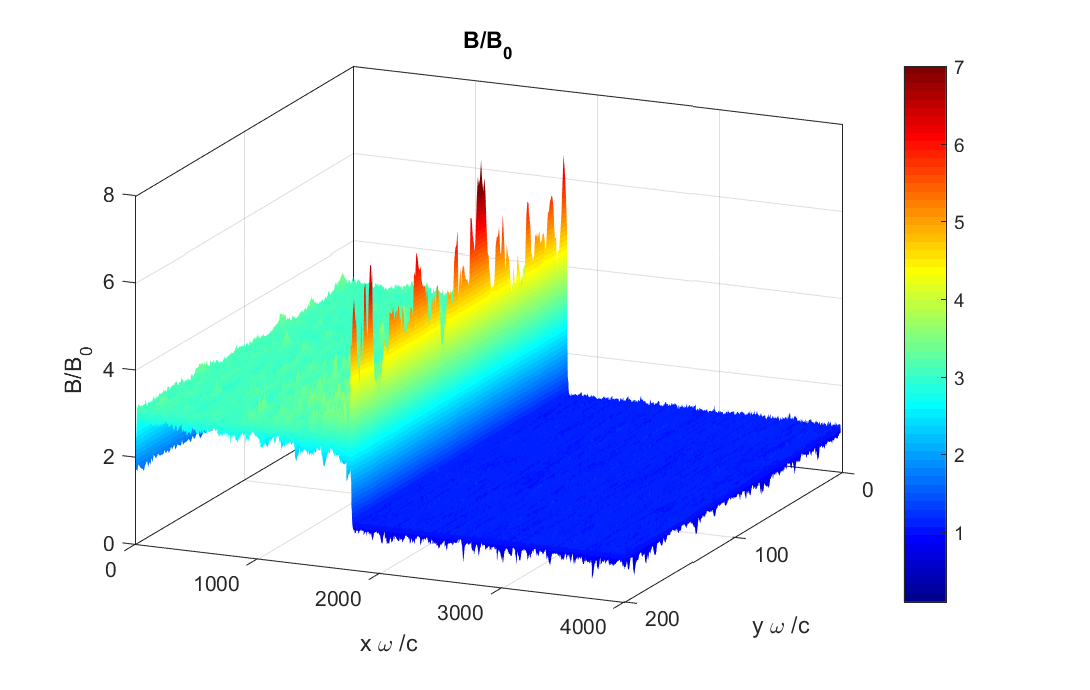
\includegraphics[width=0.7\textwidth]{fig/regular_field.eps} 
		\caption{Magnetic field in shock wave without turbulence.}
		\label{regularB}
\end{figure}
\begin{figure}[h!]
		\centering
		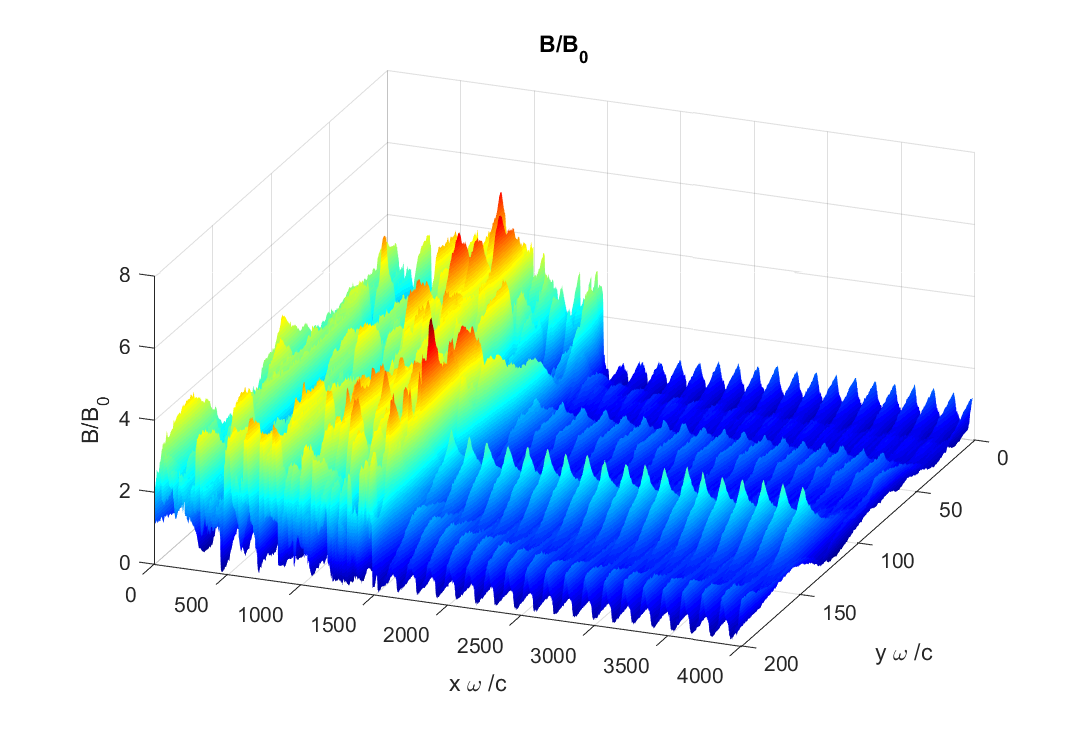
\includegraphics[width=0.7\textwidth]{fig/turbulent_field.eps} 
		\caption{Magnetic field in shock wave with 90\% turbulence.}
		\label{turbulentB}
\end{figure}
The spectrum of accelerated electrons  shown in Figure \ref{spectrum}  demonstrated a strong dependence on the fraction of the turbulent magnetic 
field energy density in the wind. 
When a half of the magnetic field energy density is in the magnetic turbulence the particle spectrum becomes significantly 
different from the spectrum in a homogeneous field. A fraction of the accelerated electrons highly increases with the growth of turbulent energy fraction. 
The quantity which is showing how much of the upstream flow kinetic energy (or the ram pressure) goes to the accelerated electrons 
$\epsilon_e$ can be defined as that in \cite{Crumley2019}
\begin{equation}
\epsilon_e = \frac{\int_{p_{inj}}^{\infty}E(p)F(p)dp}{\int_{0}^{\infty}E(p)F(p)dp }\frac{m_e(\langle \gamma \rangle - 1)}{m_p (\gamma_0 - 1)}
\end{equation}
where $F(p)$ is the electron distribution function, $E(p)$ is the energy of a particle of momentum $p$ and $\langle \gamma \rangle$ is the averaged Lorentz-factor. 
$p_{inj}$ is injection momentum, showing that particle is non-thermal and we consider it equal to $2 \gamma_0 \beta_0 m_p c$. For simulation with the strongest turbulence, $\epsilon_e$ is equal to $2\cdot10^{-3}$, and it is several times higher then that in a quasi-parallel shock wave.
\begin{figure}[h!]
	\centering
	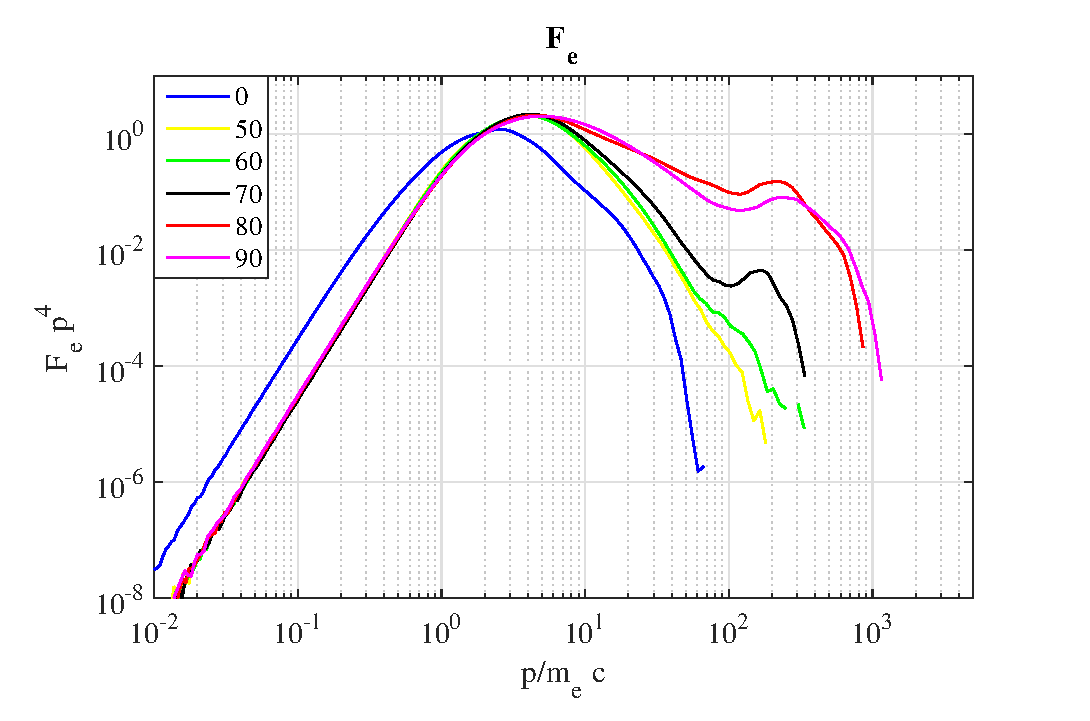
\includegraphics[width=0.7\textwidth]{fig/spectrum.eps} 
	\caption{Distribution of electrons in the relativistic shock wave with different turbulence fractions.}
	\label{spectrum}
\end{figure} 

The spectrum of accelerated electrons also depends on the scales of magnetic turbulence. We tested a few setups with different maximal wave length of the magnetic turbulent modes, corresponding to the minimal wavenumber $k_{min} = 2 \pi / 5 r_g$, $2 \pi / 10 r_g$ and $ 2 \pi /20 r_g$. As it is shown in Figure \ref{spectrum_length} the acceleration efficiency is somewhat higher for larger scales of fluctuations, but this dependence is weak and the spectrum changes are not very significant.

\begin{figure}[h!]
	\centering
	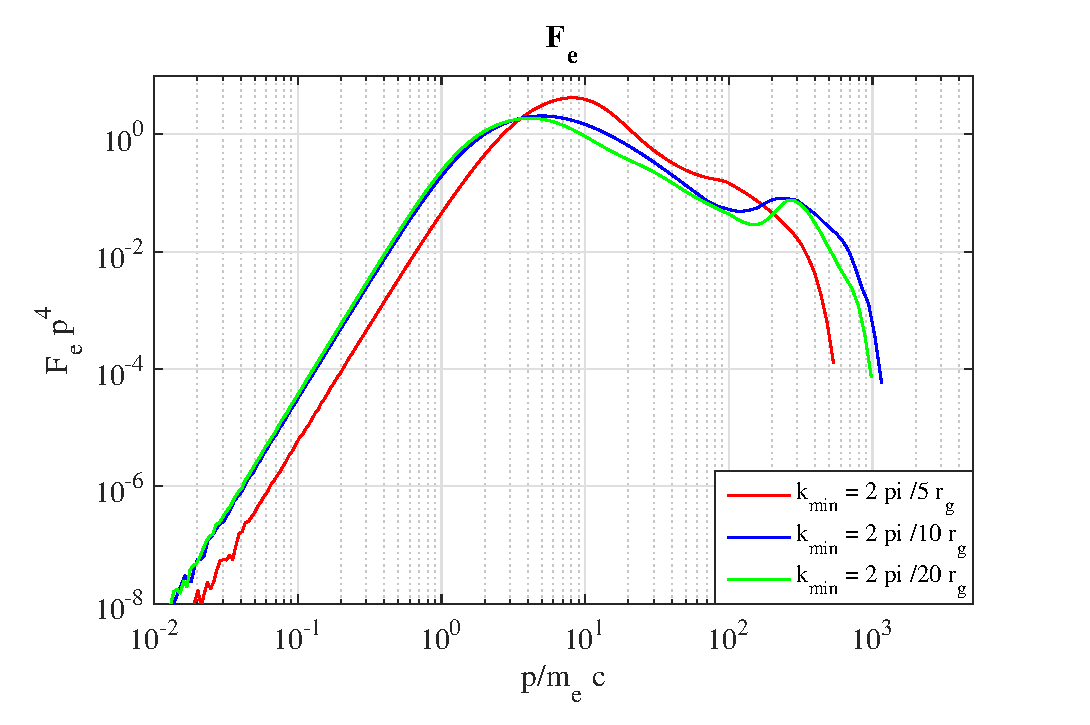
\includegraphics[width=0.7\textwidth]{fig/spectrum_length.eps} 
	\caption{Distribution of electrons in the relativistic shock wave with different turbulence length, turbulence energy fraction is 90\%.}
	\label{spectrum_length}
\end{figure} 

We tested setup with a longer transverse size of the simulation region, corresponding to approximately $40$ gyroradii of the upstream protons, with the magnetic turbulence energy fraction 90\%. The spectrum of the accelerated electrons has no qualitative differences from the setup with a smaller transverse size since the non-thermal part of the distribution function survives.  We also studied the effect of the proton to electron  mass ratio within a setup with  $\frac{m_p}{m_e} = 50$. The spectrum obtained has a similar dependence on the turbulence energy fraction and scale. It is shown in Figure \ref{electrons_mass} that the electron spectrum in the higher mass ratio setup is just shifted to the higher Lorentz-factors, while  the fraction of the energy in accelerated electrons  $\epsilon_e = 2.5\cdot10^{-3}$ is almost the same as in the case with $\frac{m_p}{m_e} = 25$.

\begin{figure}[h!]
	\centering
	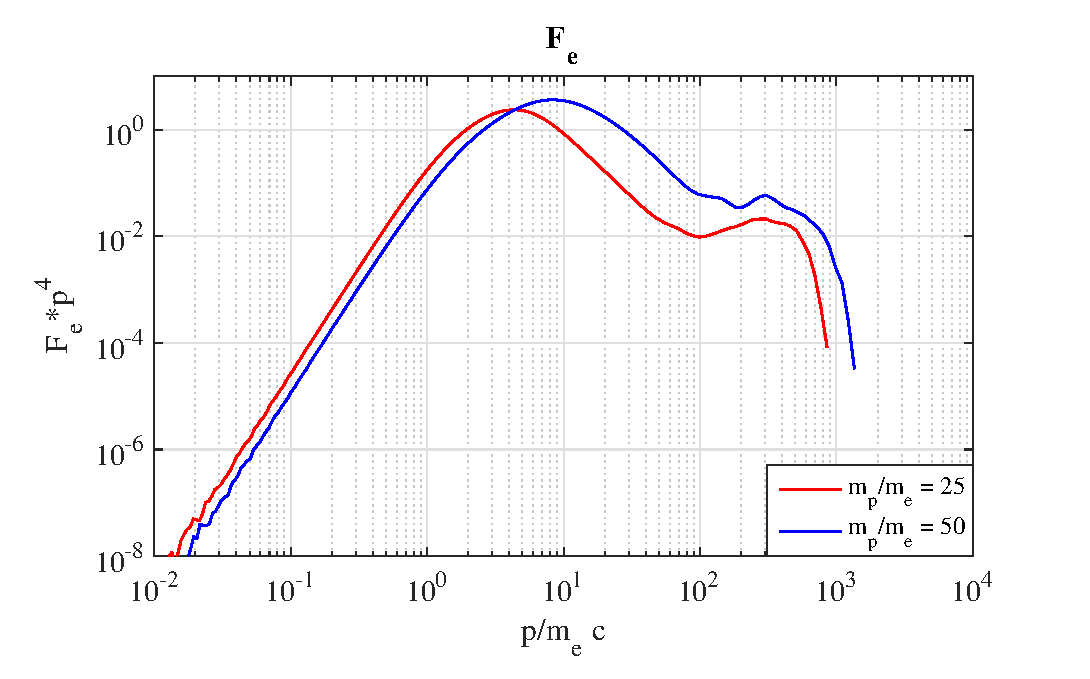
\includegraphics[width=0.7\textwidth]{fig/electrons_mass.eps} 
	\caption{Distribution of electrons in the relativistic shock wave with different mass relation, turbulence energy fraction is 90\%.}
	\label{electrons_mass}
\end{figure} 

\section{Conclusions}
In this paper we presented the results of particle-in-cell simulation of electron acceleration in trans-relativistic shock propagating in a clumped  wind of a massive star. Simulations show that the presence  of background  magnetic turbulence in the clumped wind has strong impact on particle acceleration and the acceleration is efficient for high enough level of the magnetic turbulence. The electron acceleration is highly suppressed in the case of  trans-relativistic shock propagating quasi-perpendicular to a regular magnetic field in the wind without the background magnetic turbulence. With the PIC simulations we demonstrated here that the presence of magnetic fluctuations in the background wind results in efficient electron acceleration by the quasi-perpendicular trans-relativistic shocks. We find that the scales and amplitudes of the magnetic turbulent field are important for this process. Further PIC simulations with a wider dynamical range will allow to study the effect of turbulent wind on particle acceleration in detail.

\ack
The authors acknowledge a support from RSF grant 16-12-10225.


%\newpage

\section*{References}

\bibliographystyle{iopart-num}
\bibliography{bibliogr}
\end{document}